\documentclass{swp1}
\usepackage[utf8]{inputenc}
\usepackage{amssymb}
\usepackage{url}


% Tabellen
\usepackage{tabularx}
\usepackage{supertabular}
\usepackage{booktabs}







\begin{document}

% \maketitle{Nummer}{Abgabedatum}{Tutor-Name}{Gruppennummer}
%           {Teilnehmer 1}{Teilnehmer 2}{Teilnehmer 3}
\maketitle{3}{29.06.2014}{Michaela Bunke}{ChronoX}
          {Tim Ellhoff}{Karsten Betjemann}{}
          
\section*{Aufgabe 1)}

Der Anwendungsfall dieser Aufgabe lässt sich am einfachsten anhand des zentralen Prozesses \emph{Einschreibung an der Universität} schlicht nach diesem benennen.\newline
In Bezug auf diesen Anwendungsfall gibt es drei interagierende Akteure zu benennen, wobei mit StudentIn und SachbearbeiterIn die beiden grundsätzlich am Prozess beteiligten Akteure gelistet sind und es als eine spezifische Untergruppe von StudentIn auch noch die Variation InternationaleR StudentIn gibt.\newline
Der Prozess selbst wird unter der Bedingung eingeleitet, dass vonseiten eines Studenten Interesse an der Einschreibung an der Universität besteht, sowie dass eine Sachbearbeiterin zur Bearbeitung der Aufgabe zur Verfügung steht und auf sämtliche notwendigen Systeme und Daten zugegriffen werden kann.\newline
Beim eigentlichen Prozessablauf tätigen Mitarbeiter und Student die Einschreibung dergestalt gemeinsam, als dass die für die Einschreibung nötigen Informationen vom Studenten an die Mitarbeiterin ausgegeben werden, die die Einschreibung vornimmt, zuletzt kann auch eine Einschreibung für einen Studiengang durchgeführt werden, auch wenn dies nicht notwendigerweise Teil des Prozessablaufs sein muss.Die Einschreibung für ein Stduium Generale steht in einer Vererbungsbeziehung zur Einschreibung an der Universität und in dieser Hinsicht in Beziehung zu diesem Prozessablauf.\newline
Die nenneswerte Variation im Prozessablauf basiert auf der Vorbedingung dass der Akteur StudentIn der Gruppe InternationaleR StudentIn zugeordnet ist, in diesem Falle kann von jener Seite aus zuvor eine Stellungnahme des International Office als zusätzlich für den Prozess anwendbarer Datensatz eingeholt werden.

\section*{Aufgabe 2)}

Zur Auswertung der in der Aufgabe gelisteten Szenarien bietet sich ein Vorgehen nach dem Schema der klassischen textuellen Beschreibung von Anwendungsfällen an, wobei einleitend gesagt sei dass die in den Szenarien gelisteten Nutzfälle der Informationssuche durch Privatkunden und Großkunden, sowie der Händlerbestellung und Direktbestellung entsprechen, wobei als beteiligte Akteure Privatkunde,Großkunde,Händler,Disponent zu listen sind.\newline
\newline
\emph{Szenario 1}\newline
\textbf{Name:}\newline
Informationszugriff und Konfiguration - Privatkunde\newline
\textbf{Akteure:}\newline
Privatkunde\newline
\textbf{Vorbedingung:}\newline
Privatkunde wünscht Informationen zu spezifischem Produkt\newline
Privatkunde hat Zugang zum Informationssystem\newline
Informationssystem ist einsetzbar/verfügbar\newline
\textbf{Nachbedingung:}\newline
Privatkunde hat eigene Produktkonfiguration erstellt\newline
\textbf{Ablauf:}\newline
Privatkunde greift auf das Informationssystem zu\newline
Privatkunde sucht nach dem Modell X123\newline
Informationssystem zeigt Kenndaten von Modell X123 an\newline
Privatkunde konfiguriert Kenndaten im Sinne eines Wunschmodells\newline
\newline
\emph{Szenario 2}\newline
\textbf{Name:}\newline
Informationszugriff - Großkunde\newline
\textbf{Akteure:}\newline
Großkunde\newline
\textbf{Vorbedingung:}\newline
Großkunde wünscht Informationen über spezifisches Modell\newline
Großkunde hat Zugang zum Informationssystem\newline
Informationssystem ist einsetzbar/verfügbar\newline
\textbf{Nachbedingung:}\newline
Keine Nachbedingung\newline
\textbf{Ablauf:}\newline
Großkunde greift auf das Informationssystem zu\newline
Großkunde sucht nach dem Modell X987\newline
Informationssystem zeigt Kenndaten von Modell X987 an\newline
Großkunde sucht nach dem Modell X567\newline
Informationssystem zeigt Kenndaten von Modell X567 an\newline
Großkunde beendet das Informationssystem\newline
\newline
\emph{Szenario 3}\newline
\textbf{Name:}\newline
Händlerbestellung - Privatkunde\newline
\textbf{Akteure:}\newline
Privatkunde\newline
Händler\newline
Disponent\newline
\textbf{Vorbedingung:}\newline
Privatkunde möchte ein Modell bestellen\newline
Händler ist verfügbar\newline
Disponent ist verfügbar\newline
Informationssystem/Bestellsystem ist verfügbar\newline
Produktionssystem ist verfügbar\newline
\textbf{Nachbedingung:}\newline
Bestellung ist abgeschlossen\newline
Produktionsauftrag ist erstellt\newline
\textbf{Ablauf:}\newline
Privatkunde sucht Händler auf\newline
Händler erhält Bestelldaten von Privatkunde\newline
Händler ruft Informationssystem/Bestellsystem auf\newline
Händler sucht nach Modell X234\newline
Informationssystem/Bestellsystem zeigt Datenblatt zu Modell X234 an\newline
Händler konfiguriert das Modell nach den Wunschdaten des Kunden\newline
Händler nutzt integriert Bestellfunktion zur Bestellung von Modell X234\newline
Informationssystem/Bestellsystem leitet Bestellauftrag an Disponenten weiter\newline
Disponent bestätigt Bestellung und schließt damit die Bestellung ab\newline
Händler beendet Informationssystem/Bestellsystem\newline
Disponent ruft Produktionssystem auf\newline
Disponent erstellt Produktionsauftrag\newline
Disponent beendet Produktionssystem\newline
\newline
\emph{Szenario 4}\newline
\textbf{Name:}\newline
Direktbestellung - Großkunde\newline
\textbf{Akteure:}\newline
Großkunde\newline
Händler\newline
Disponent\newline
\textbf{Vorbedingung:}\newline
Großkunde möchte ein Modell bestellen\newline
Alle haben Zugriff auf das Informationssystem/Bestellsystem\newline
Informationssystem/Bestellsystem ist verfügbar\newline
Disponent hat Zugriff auf Produktionssystem\newline
Produktionssystem ist verfügbar\newline
\textbf{Nachbedingung:}\newline
Bestellung ist abgeschlossen\newline
Produktionsauftrag ist erstellt\newline
\textbf{Ablauf:}\newline
Großkunde ruft Informationssystem/Bestellsystem auf\newline
Großkunde sucht nach Wunschmodell\newline
System zeigt Datenblatt an\newline
Großkunde konfiguriert die Modelldaten nach Wunsch\newline
Großkunde gibt Bestellung auf\newline
Händler und Disponent bestätigen Bestellung\newline
Disponent ruft Produktionssystem auf\newline
Disponent gibt Produktiuonsauftrag aus\newline
\newline
Alle Szenarien lassen sich einem Anwendungsfalldiagramm darstellen um den Prozessablauf schematisch zu überlicken und zu verdeutlichen.\newline
\newline
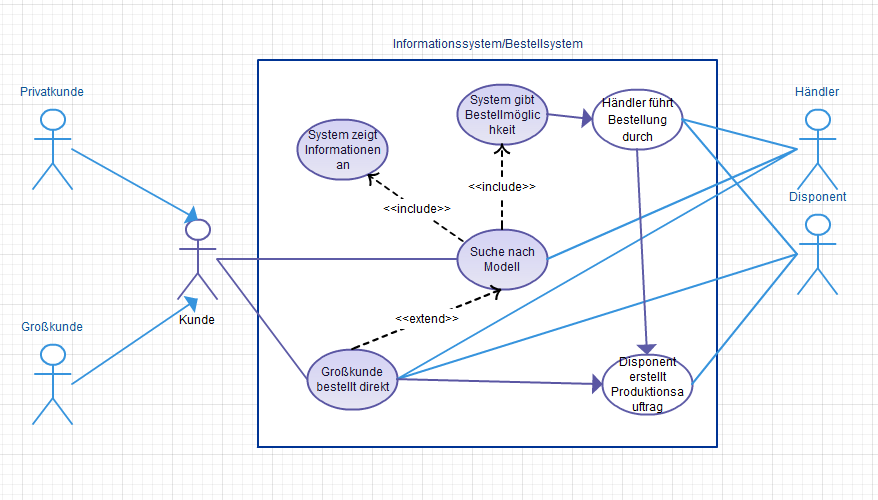
\includegraphics[scale=0.75]{Diagramm}
\newline

\section*{Aufgabe 3)}

\textbf{Assoziation:}\newline
Assoziationen sind eine Relation, welche in UML Klassendiagrammen angewandt wird um eine Beziehung zwischen mehreren Objektinstanzen anzuzeigen.
Besondere Bedeutung hat hierbei der Umstand, dass diese Assoziationen auch eine Navigierbarkeit implizieren können, was gestalterisch durch Pfeile anzeigbar ist.\newline
Diese Navigierbarkeit ist notwendig um im Rahmen der Implementierung erkennen zu können ob irgendwo ein Wechsel vom Einem Objekt zum Anderen realisiert werden muss und ist zum Beispiel durch die Speicherung einer Objektreferenz in einem Attribut umsetzbar.\newline
\textbf{Aggregation:}\newline
Die Aggregation kann als speziellere Form der Assoziation verstanden werden, welche dazu dient eine vereinigende Beziehung von einzelnen Objekten in einem Aggregat zu symbolisieren.
Durch diese Maßnahme lassen sich also übergeordnete Aggragate aus unterschiedlich vielen Objekten bilden, um so eine bessere Ordnung oder eine genauere Spezifikation zu ermöglichen.\newline
Eine beispielhafte Möglichkeit hierfür wäre die Unterordnung verschiedener Bücher in eine Buchreihe.\newline
\textbf{Komposition:}\newline
Die Komposition lässt sich leicht als erweiterte und stärkere Form der Aggregation verstehen, wobei hier signalisiert wird, dass das Aggregat und seine Komponenten logisch derartig miteinander verbunden sind, als dass die Komponenten selbst nicht ohne das Aggregat vorhanden sein können, es existiert also eine ständige und starke Bindung zwischen beiden, diese beruht auch darauf, dass eine Komposition nur zwischen den Komponenten und jeweils einem Aggregat bestehen kann.\newline
Als logisches Beispiel könnte man eine Buchreihe durch Komposition mit einem Verlag darstellen, um zu signalisieren das eine Buchreihe nicht ohne den dazugehörigen Verlag exisitieren kann, auch wenn diese Beispiel im Zusammenhang mit der modernen Eigenpulikation vielleicht an Schärfe verlieren kann.\newline
\textbf{Generalisierung:}\newline
Generalisierungen sind eine praktische Relation zur Umsetzung von Vererbungshierarchien auf der schematischen Ebene von Oberen und Unteren Klassen, sie kennzeichnen voneinander erbende Klassen und geben gleichzeitig die Richtung in der Erbhierachie an, wobei die Unteren Klassen die Attribute und Methoden der Oberen Klassen erben, selbige aber auch beliebig umschreiben und erweitern oder aber auch neue Methoden und Attribute definieren können. Im Rahmen der Generalisierungen können auch abstrakte Klassen angelegt werden, die nur zur Einfachheit mehrere Eigenschaften vererbbar in sich vereinigen, als Objekt angewandt jedoch nicht vorkommen.\newline
Als beispielhafte Umsetzung könnte man eine Klasse Person als abstrakte Oberklasse innerhalb des eigenen Diagramms einsetzen um hierin alle generellen Eigenschaften der in der Darstellung auftauchenden Akteure zu vereinen, sodass man für die tatsächlich beteiligten Akteure nur Rücksicht auf gesonderte Eigenschaften nehmen muss, da alle allgemeinen Eigenschaften bereits über die Vererbungshierarchie aufgeführt und in Beziehung gesetzt wurden.Damit wären Klassen wie \emph{Ausleiher} oder \emph{Bibliothekar} lediglich Subklassen von Person mit wenigen zu listenden Sondereigenschaften.

\section*{Aufgabe 4)}



\section*{Aufgabe 5)}

\textbf{a)}\newline

Die beiden Diagramme modellieren eine Lehrveranstaltung im Bezug auf die Beziehung zwischen den an der Veranstaltung teilnehmenden Personen und der Lehrveranstaltung, welche beide als Klassen realisiert sind und zwischen jenen sowie dem ebenfalls als Klasse umgesetzten Semester, in welchem die Teilnahme stattfindet.In allen Diagrammen sind dabei dieselben Klassen umgesetzt, so exisitieren gleichermaßen die Klassen \emph{Person} und \emph{Lehrveranstaltung}, die jeweils die Eigenschaften \emph{name} und \emph{titel} vom Typ String aufweisen, wie auch die Klasse \emph{Semester}, welche die Eigenschaften \emph{jahr} vom Typ Integer, sowie \emph{wiSe} vom Typ Boolean besitzt.Der vornehmlichste Unterschied zwischen den Diagrammen besteht also nicht in den existieren Klassen selbst, sondern in der Modellierung ihrer Beziehungen untereinander, hier besteht die Gemeinsamkeit nur in einer Assoziation \emph{nimmt teil an}, die von \emph{Person} nach \emph{Lehrveranstaltung} navigierbar ist.\newline
\newline
Im Rahmen eines Objektdiagramms lassen sich die zuvor besprochenen Klassenobjekte noch einmal verdeutlichen.\newline
\newline
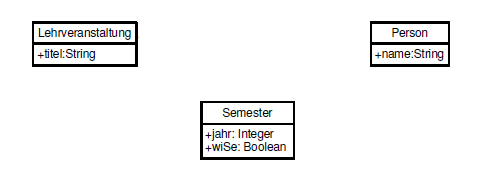
\includegraphics{Objektdiagramm}
\newline
Beim ersten Diagramm besteht diese Beziehung weiterhin auch als einzige einfache Assoziation in der Modellierung, die Klasse \emph{Semester} ist hierbei nämlich als Assoziationsklasse an die Beziehung \emph{nimmt teil an} angegliedert, weitere Assoziationen bestehen in der Darstellung nicht. Diese Form der Modellierung einer mehrstelligen Assoziation ist dann praktisch, wenn gewünscht wird eine Beziehung mit Attributen zu versehen und damit eine Beziehung zu beschreiben, welche gleichzeitig die Funktion einer Klasse einnimmt, um so die Klassen \emph{Person} und \emph{Lehrveranstaltung} in eine spezifischere Beziehung zu setzen.\newline
Ein Beispiel für diese Umsetzung ließe sich folgendermaßen gestalten,
\newline
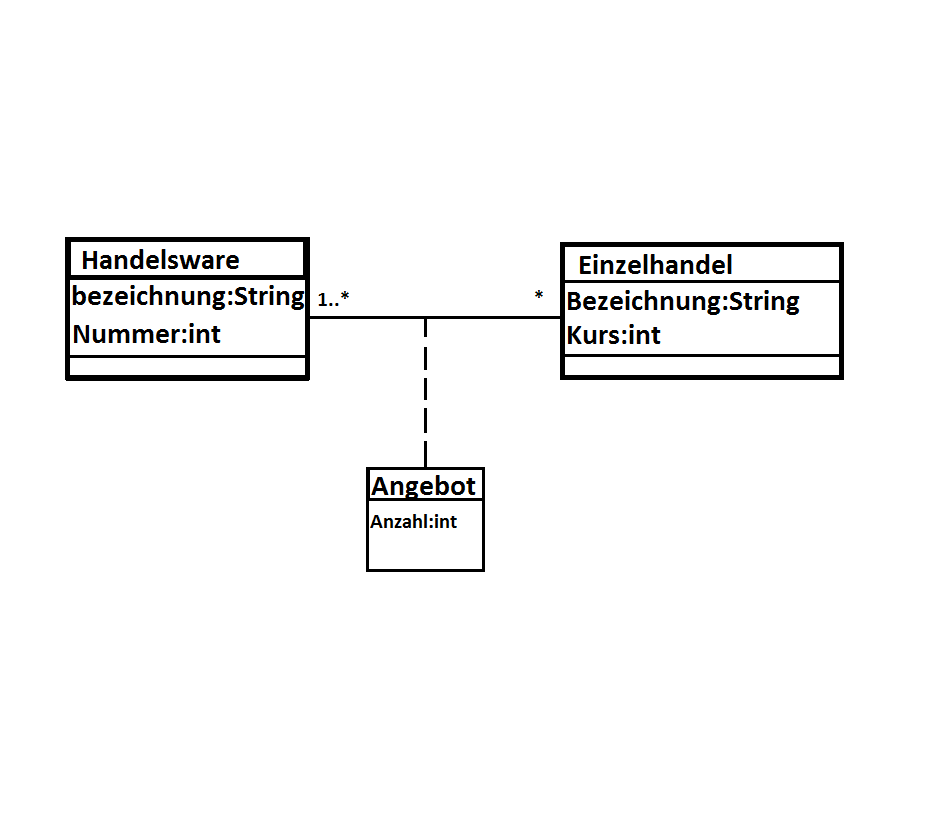
\includegraphics[scale=0.5]{Assoziationsklasse}
\newline
Somit werden in dieser Modellierung die Attribute von \emph{Semester} direkt der Assoziation \emph{nimmt teil an} zugeordnet, was einerseits die Übersichtlichkeit in der Darstellung erhöht, vor allem aber das Abrufen der Attribute im Rahmen der Assoziation ermöglicht, statt eine neue Assoziation zur Klasse \emph{Semester} anlegen und abrufen zu müssen.\newline
\newline
Das zweite Diagramm gestaltet sich in dieser Hinsicht anders, da es auf eine Assoziationsklasse verzichtet und stattdessen die Klasse \emph{Semester} als seperate Klasse realisiert, welche in ihre Richtung navigierbare Assoziationen zwischen ihr und der Klasse \emph{Lehrveranstaltung}, in Form der Assoziation \emph{findet statt in}, und der Klasse \emph{Person}, über die Assoziation \emph{nimmt teil in} aufweist.\newline
Diese Darstellung bettet die Attribute der Klasse \emph{Semester} nicht in den Rahmen einer Assoziation ein, sondern verknüpft sie mit den beiden anderen Klassen über jeweils eine gesonderte Assoziation, eine Modellierung, welche sich im Ausbau auch als Realisierung einer mehrstelligen Assoziation durch den Einsatz einer verbindenden Klassen anwenden lässt.Dieser eher klassische Ansatz erlaubt es dann nach folgendem Beispiel mehrere Klassen zugleich miteinander zu assoziieren.\newline
\newline
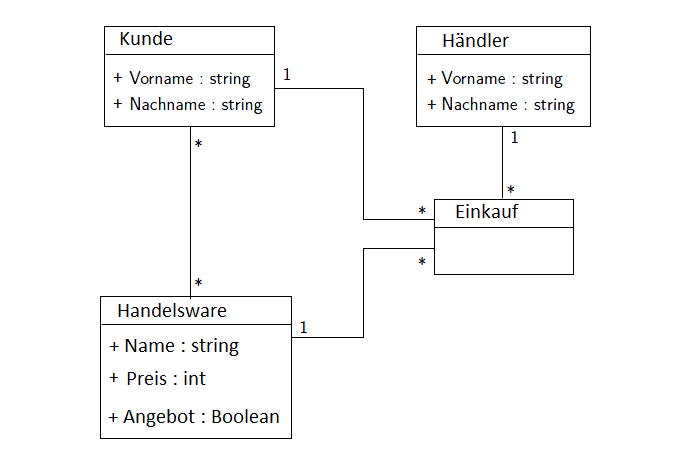
\includegraphics[scale=0.5]{Mehrteilige_Assoziation}
\newline
Konkret unterscheidet sich diese Darstellungsform dahingehend, als dass die Attribute von \emph{Semester} eben nicht nur einer Assoziation zugeordnet werden, sondern über seperate Beziehungen abgerufen werden können, was je nach Interessenslage gefragt sein kann.\newline

\textbf{b)}\newline

Gehen wir von der Annahme aus, dass die Attributierung von \emph{Semester} im Rahmen der Assoziation \emph{nimmt teil an} gefragt ist, so würde ich mich definitiv für die erste Modellierungsvariante entscheiden, da diese eine klare Zuordnung jener Klasse zur Beziehung selbst kennzeichnet. Auf diese Weise ist in übersichtlicher Weise dargestellt dass im Rahmen der eigentlichen Beziehung der Teilnahme bereits ein Mechanismus zum Abrufen der Attribute zu implementieren ist.\newline
Da auch eine Assoziaitonsklasse noch mit weiteren Klassen assoziert werden kann ist hier auch noch eine weitere Verknüpfung möglich, falls der gesamte Fall ausgebaut werden muss, auch wenn hier die Realisierung als mehrstellige Assoziation über eine Klasse übersichtlicher sein könnte.

\section*{Aufgabe 6)}

Das vorliegende Klassendiagramm weist mehrere Mängel auf, so sind die Multiplizitäten der einzelnen Assoziationen nicht angegeben wodurch die Standarmultiplizität 1 bei einer Verbindung zu vielen Objekten wie bei der Klasse \emph{Gruppe} irreführend, ebenso sind die Assoziationen nicht benannt und weisen keine definierten Rollen auf, auch ließe sich die Aggregation zwischen \emph{TutorIn} und \emph{Lehrkraft} anders modellieren und Irreführung zu vermeiden und zuletzt sollten Atrribute in der Regel versteckt werden, statt in Klassendiagrammen zu Entwurf oder Implementierung öffentlich sichtbar zu sein.

\section*{Aufgabe 7)}




\end{document}

